\documentclass[11pt,a4paper]{article}
\usepackage[T1]{fontenc}
\usepackage[margin=2.3cm]{geometry}
\usepackage{amsmath,amssymb}
\usepackage{graphicx}
\usepackage[dvipsnames]{xcolor}
\usepackage{enumitem}
\usepackage[colorlinks=true,linkcolor=blue,urlcolor=blue]{hyperref}
\setlength{\parskip}{0.6em}
\setlength{\parindent}{0pt}
\begin{document}

\begin{center}{\LARGE\bfseries openhousehold}\\[0.4em]{\large Predict your home's electricity bill, and see where every kilowatt-hour goes.}\\[0.2em]\small PAN IIT OSS explainer \textbullet{} middle school to higher secondary (levels 2-4)\end{center}

\section*{Why this exists}
Every home is a small power system: appliances that draw power at different hours, a meter that adds it up into energy, and a tariff that turns energy into money. This explainer shows how to model that with multiplication, a 24-hour profile and a little randomness.

\section*{The end goal}
Predict a household's daily electricity use and bill, and see where the energy goes. The end goal is to predict a household's daily electricity use and bill, and to see where the energy goes, including the effect of rooftop solar. The same thinking supports energy audits, tariff design and sizing of home solar systems.

\section*{How the three sessions build up}
\begin{enumerate}[nosep]
\item \textbf{Session 1: Power times time is energy} (Level 1, conceptual interactive model, 60 min).
\item \textbf{Session 2: A day of load and a bill with slabs} (Level 2, mathematical engineering model, 75 min).
\item \textbf{Session 3: A month with random usage and rooftop solar} (Level 3, simulation and validation, 90 min).
\end{enumerate}

\section{Session 1: Power times time is energy}

\subsection*{A. Real-world problem}
An electricity bill is in 'units'. A 1500 W water heater feels powerful, yet a 100 W TV left on for the whole evening also costs money. Which one matters more? The answer depends on both how strong an appliance is (power) and how long it runs (time). This session gives you the one rule that turns a list of appliances into a number of units and a cost. Education only: a simplified model, not advice about wiring or buying appliances.

\subsection*{B. Concept and theory}
Power is how fast energy is used. Its unit is the watt (W); 1 kilowatt (kW) is 1000 W. Energy is the total used over some time. When power is in kW and time in hours, energy comes out in kilowatt-hours (kWh), the 'unit' on your bill. The cost is the energy times the price per kWh (the rate). Energies of different appliances can simply be added.

\begin{itemize}[nosep]
\item P: power of an appliance (W or kW)
\item t: time the appliance is switched on (h)
\item E: energy used (kWh)
\item r: price of energy (flat, illustrative) (Rs per kWh)
\item C: cost (Rs)
\end{itemize}

\begin{equation*}
E\,[\mathrm{kWh}]=P\,[\mathrm{kW}]\times t\,[\mathrm{h}]
\end{equation*}

\begin{equation*}
E_{\mathrm{day}}=\sum_i P_i\,t_i
\end{equation*}

\begin{equation*}
C=E_{\mathrm{day}}\times r
\end{equation*}

\begin{center}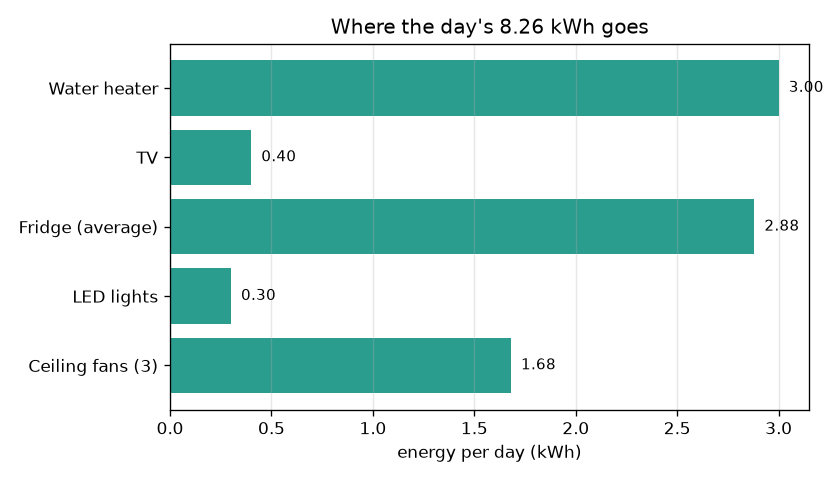
\includegraphics[width=0.85\linewidth]{figures/s01_daily_energy_bars.png}\\\small Energy per appliance per day: the heater and the always-on fridge lead.\end{center}

\subsection*{E. Worked example}
A 1.5 kW heater runs for 2 hours. How much energy does it use? What if the time is halved? What does the whole household of the app use per day and what does it cost at Rs 6 per kWh?
\begin{enumerate}[nosep]
\item Heater: E = 1.5 kW x 2 h = 3 kWh.
\item Half the time: E = 1.5 kW x 1 h = 1.5 kWh. Half the time, half the energy.
\item Others: fans 0.21 kW x 8 h = 1.68 kWh; lights 0.06 kW x 5 h = 0.30 kWh; fridge 0.12 kW x 24 h = 2.88 kWh; TV 0.10 kW x 4 h = 0.40 kWh.
\item Total = 1.68 + 0.30 + 2.88 + 0.40 + 3.00 = 8.26 kWh per day.
\item Cost = 8.26 kWh x Rs 6 = Rs 49.56 per day. With the heater at 1 hour the total is 6.76 kWh and Rs 40.56, a saving of Rs 9.00 a day.
\end{enumerate}
\textbf{Answer.} The heater uses 3 kWh, or 1.5 kWh if the time is halved. The household uses 8.26 kWh and pays Rs 49.56 per day at Rs 6 per kWh.

\subsection*{F. Questions}
\begin{enumerate}[nosep]
\item \textbf{Conceptual.} Explain the difference between a kilowatt and a kilowatt-hour. Which one does the bill charge for?
\item \textbf{Numerical.} A 100 W TV runs for 4 hours a day. Find its energy per day and per 30 days, and the cost per 30 days at Rs 6 per kWh. Check that the answer is sensible.
\item \textbf{Graph and simulation interpretation.} In the straight-line graph of heater energy against time, what does the slope mean? What happens to the line if you halve the power?
\item \textbf{Design and optimisation challenge.} Design: the family wants the daily cost under Rs 40 (it is Rs 49.56 now) without giving up hot water entirely. List two changes from the app and check each with a calculation.
\end{enumerate}

\section{Session 2: A day of load and a bill with slabs}

\subsection*{A. Real-world problem}
Two homes can use the same number of units in a month and yet one needs thicker wires and a bigger supply because it switches everything on at the same time. And a bill is rarely 'units times one price': in a slab tariff, the price per unit steps up as you use more. A family wants to cut its bill by 20 percent. How much less must it use? The tariff here is an illustrative teaching tariff, not any real utility's, and this is a simplified model, not an electrical design tool.

\subsection*{B. Concept and theory}
Divide the day into 24 hours. In each hour the home's power is the sum of the powers of the appliances that are on. Because one hour at P kW is P kWh, the daily energy is the sum of the 24 hourly powers. The peak demand is the largest hourly power. The monthly energy is 30 times the daily energy. A slab tariff charges a fixed amount plus a different rate for each band of units: here 3 Rs per kWh for the first 100 kWh, 5 Rs for the next 100 and 7.5 Rs above 200, plus Rs 50 a month. In alternating current, only the real power P does useful work and is billed as energy, but the current also depends on the power factor pf: apparent power S = P / pf (in kVA) and current I = P / (V x pf).

\begin{itemize}[nosep]
\item P(h): home power in hour h (kW)
\item E\_day: energy per day (kWh)
\item E\_m: energy per month (30 days) (kWh)
\item P\_peak: largest hourly power (kW)
\item pf: power factor, 0 to 1 (no unit)
\item S: apparent power (kVA)
\item V: supply voltage (230) (V)
\item I: current at the peak (A)
\end{itemize}

\begin{equation*}
P(h)=\sum_{i} P_i(h),\qquad E_{\mathrm{day}}=\sum_{h=0}^{23} P(h)\times 1\,\mathrm{h}
\end{equation*}

\begin{equation*}
\mathrm{bill}=50+3\min(E_m,100)+5\min\big(\max(E_m-100,0),100\big)+7.5\max(E_m-200,0)
\end{equation*}

\begin{equation*}
S=\frac{P}{\mathrm{pf}},\qquad I=\frac{P\times 1000}{V\,\mathrm{pf}}
\end{equation*}

\begin{center}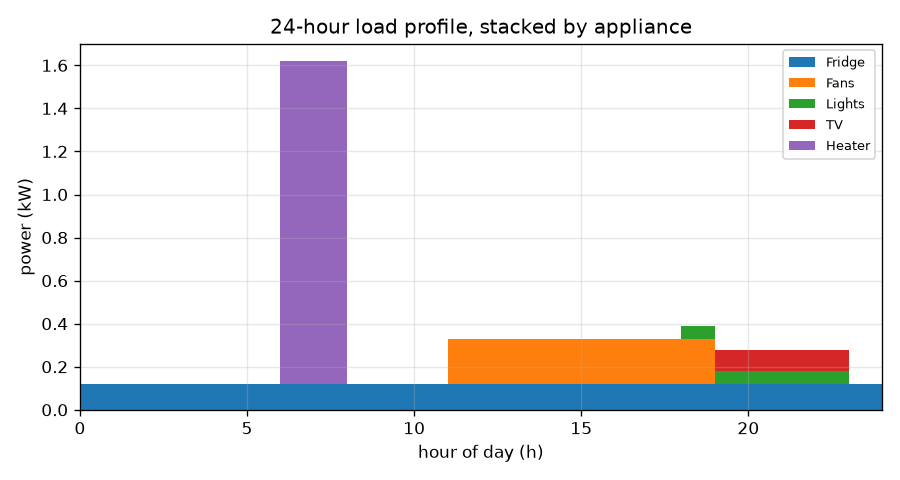
\includegraphics[width=0.85\linewidth]{figures/s02_load_profile.png}\\\small Hourly load stacked by appliance; the heater makes the 1.62 kW peak at 6 to 8.\end{center}

\subsection*{E. Worked example}
With the heater on from 6:00 for 2 hours, find the daily energy, the monthly energy, the monthly bill, the peak demand, and the current at the peak for pf 0.9 on 230 V.
\begin{enumerate}[nosep]
\item Daily energy: fridge 2.88 + fans 1.68 + lights 0.30 + TV 0.40 + heater 3.00 = 8.26 kWh.
\item Monthly energy = 30 x 8.26 = 247.8 kWh.
\item Slab bill: 50 + 100 x 3 + 100 x 5 + (247.8 - 200) x 7.5 = 50 + 300 + 500 + 358.5 = Rs 1208.50.
\item Peak: in hours 6 and 7 the fridge (0.12 kW) and heater (1.5 kW) are on: 1.62 kW.
\item At pf 0.9: S = 1.62 / 0.9 = 1.80 kVA and I = 1620 / (230 x 0.9) = 7.83 A.
\end{enumerate}
\textbf{Answer.} 8.26 kWh per day, 247.8 kWh per month, a bill of Rs 1208.50, a peak of 1.62 kW (1.80 kVA, 7.83 A).

\subsection*{F. Questions}
\begin{enumerate}[nosep]
\item \textbf{Conceptual.} Why can two homes with the same monthly kWh have different peak demand? Why does the peak matter even though the bill is only for kWh?
\item \textbf{Numerical.} A home uses 150 kWh in a month. Find its bill with the slab tariff and its average price per kWh. Check that the answer is sensible.
\item \textbf{Graph and simulation interpretation.} On the bill graph, how much more does 10 extra kWh cost at 250 kWh than at 50 kWh? Why?
\item \textbf{Design and optimisation challenge.} Design: cut the monthly bill from Rs 1208.50 by 20 percent. Find the heater time needed if nothing else changes, then find a second plan that also cuts the fans, lights and TV by 20 percent. State the energy cut each needs and the trade-offs.
\end{enumerate}

\section{Session 3: A month with random usage and rooftop solar}

\subsection*{A. Real-world problem}
A family is thinking about a rooftop solar array. Will it cut the bill? By how much? Weather and habits change every day, so one number cannot be exact. We simulate a whole month many times, subtract the sun's power hour by hour, and ask how the bill responds to the size of the array, the tariff and the usage. And we check the simulation against a calculation by hand, so we know when to trust it. This is general education with an illustrative tariff, not a quotation or a design for any real installation.

\subsection*{B. Concept and theory}
Each day the load is the Session 2 profile, but the heater time is multiplied by a random factor between 0.5 and 1.5 and the other habits by a random factor between 0.8 and 1.2. Solar generation is a half sine between 6:00 and 18:00 with peak power kWp x derate, scaled by a random cloud factor (average 0.85). Derate (0.6) lumps together heat, wiring, inverter and dust losses. Each hour the home imports energy if the load exceeds the solar power and exports if it is lower. With net metering the month is billed on imports minus exports, never below zero (extra credit is carried forward, not paid out, in this model). Without export credit the bill is based on imports only.

\begin{itemize}[nosep]
\item kWp: peak rating of the array (kW)
\item derate: fraction of the rating actually delivered (0.6) (no unit)
\item c: cloud factor of the day (no unit)
\item G(h): solar power in hour h (kW)
\item L(h): home load in hour h (kW)
\item Imp, Exp: monthly imported and exported energy (kWh)
\item N: net energy billed (kWh)
\end{itemize}

\begin{equation*}
G(t)=\mathrm{kWp}\cdot d\cdot c\cdot\sin\!\left(\frac{\pi (t-6)}{12}\right),\quad 6<t<18
\end{equation*}

\begin{equation*}
\mathrm{Imp}=\sum \max(L-G,0),\quad \mathrm{Exp}=\sum \max(G-L,0),\quad N=\max(\mathrm{Imp}-\mathrm{Exp},0)
\end{equation*}

\begin{equation*}
\sum_{k=0}^{11}\sin\frac{(k+1/2)\pi}{12}=\frac{1}{\sin(\pi/24)}=7.661\ \approx\ \int_6^{18}\sin\frac{\pi(t-6)}{12}\,dt=\frac{24}{\pi}=7.639
\end{equation*}

\begin{center}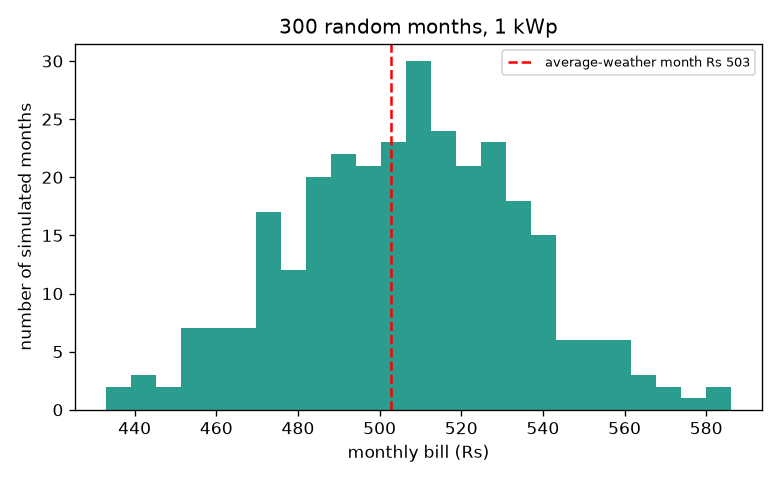
\includegraphics[width=0.85\linewidth]{figures/s03_bill_spread.png}\\\small 300 random months for a 1 kWp array: the average-weather month sits in the middle.\end{center}

\subsection*{E. Worked example}
With a 1 kWp array, average weather (cloud 0.85, no random change) and the Session 2 household, find the net energy and the monthly bill by hand and compare with the simulation.
\begin{enumerate}[nosep]
\item Sun energy per kWp per day without clouds: derate x sum of 12 midpoint sines = 0.6 x 7.661 = 4.597 kWh.
\item With cloud 0.85: 4.597 x 0.85 = 3.907 kWh per day, so 117.2 kWh in 30 days.
\item Net per day = load - generation = 8.26 - 3.907 = 4.353 kWh, so net per month = 130.6 kWh (the hourly import of 172.4 kWh minus the export of 41.8 kWh).
\item Bill: 50 + 100 x 3 + (130.6 - 100) x 5 = 50 + 300 + 153.0 = Rs 503 (Rs 502.9 with unrounded numbers).
\item Compare: no panels Rs 1208.50; without export credit Rs 711.9.
\end{enumerate}
\textbf{Answer.} Net energy 130.6 kWh and a monthly bill of about Rs 503, against Rs 1208.50 without solar. The checkpoint reproduces both numbers from the simulation.

\subsection*{F. Questions}
\begin{enumerate}[nosep]
\item \textbf{Conceptual.} Why does the bill with net metering fall by less and less for each extra half kWp of panels?
\item \textbf{Numerical.} Find the monthly net energy and the net-metering bill for a 1.5 kWp array in average weather (cloud 0.85). Check the result with the simulation.
\item \textbf{Graph and simulation interpretation.} On the bill-versus-size graph, read the bill at 0, 1, 2 and 3 kWp, and explain why the last two points are so close.
\item \textbf{Design and optimisation challenge.} Design: with a roof for at most 2 kWp, choose the smallest array (in steps of 0.5 kWp) that gives a bill of Rs 350 or less in average weather, then check it in a bad month (cloud 0.6). If exports earned nothing, would the answer still work?
\end{enumerate}

\section{Real-world mini-project}
\textbf{Audit your own home and propose three changes.} Make a list of the appliances in your home (or a relative's home, with permission): read the power in watts from the label or manual, estimate the hours of use per day, and write down the units (kWh) on one recent electricity bill. Use Session 2's functions to predict the month, compare with the bill, and propose three changes (shorter use, a different time of day, a more efficient appliance, or a rooftop array from Session 3). Do not open appliances or touch wiring; read labels and bills only. This is an education exercise, not an energy-audit certificate or financial advice.

\section{The path ahead}
\begin{enumerate}[nosep]
\item \textbf{Session 4: Fifteen-minute steps and duty cycles.} A load profile in 15-minute steps with appliances that switch on and off.
\item \textbf{Session 5: Time-of-use tariffs and load shifting.} A bill function that takes a price for each hour of the day.
\item \textbf{Session 6: Add a battery.} A battery that charges from surplus solar and discharges to cover the load.
\item \textbf{Session 7: Calibrate the model to a real meter log.} A fitting step that estimates appliance hours from seven days of meter readings.
\item \textbf{Session 8: Animate the day with a Sankey diagram.} A 48-frame GIF of the stacked load, the sun and a Sankey diagram of the flows so far.
\end{enumerate}

\section{Answers and hints}

\subsection*{Session 1}
\begin{enumerate}[nosep]
\item \textbf{Conceptual.} Hint: One is a rate, the other is an amount. Think of speed and distance. Solution: A kilowatt is power: how fast energy is being used right now (like speed). A kilowatt-hour is energy: the total used over time (like distance travelled). The bill charges for kilowatt-hours, because a strong appliance used for a few minutes can use less energy than a weak one left on all day.
\item \textbf{Numerical.} Hint: Convert watts to kW first: divide by 1000. Solution: E = 0.1 kW x 4 h = 0.4 kWh per day. Per 30 days: 0.4 x 30 = 12 kWh. Cost = 12 x 6 = Rs 72. Sanity check: a small appliance used a few hours gives only a few kWh a month, and 12 kWh fits that.
\item \textbf{Graph and simulation interpretation.} Hint: Slope is rise over run: kWh per hour. Solution: The slope is energy per hour, which is the power in kW (1.5 kWh per hour for 1500 W). Halving the power halves the slope: the line is lower and flatter, so 2 hours gives 1.5 kWh instead of 3 kWh.
\item \textbf{Design and optimisation challenge.} Hint: Cost = total energy x 6, so the total must fall below 40 / 6 = 6.67 kWh. You need to cut more than 1.59 kWh. Solution: Need 8.26 - 6.67 = 1.59 kWh or more saved. Option 1: heater 2 h to 1 h saves 1.5 kWh, not quite enough alone (6.76 kWh, Rs 40.56). Add: fans 8 h to 6 h saves 0.42 kWh. New total 6.34 kWh, cost Rs 38.04. Trade-off: less hot water and less cooling. Option 2: a 750 W heater for 2 h gives 1.5 kWh (saves 1.5 kWh too), but it heats the water more slowly, so it may need longer.
\end{enumerate}

\subsection*{Session 2}
\begin{enumerate}[nosep]
\item \textbf{Conceptual.} Hint: Think of one home that switches on everything at once and one that spreads the use. Solution: Energy adds up power over time, the peak is the highest power at one moment. A home that runs the heater, iron and cooler together has a high peak; one that staggers them has the same energy but a lower peak. The peak decides the current in the wires and the size of the supply, which must not be exceeded, even though the bill only counts kWh.
\item \textbf{Numerical.} Hint: 50 fixed, 100 kWh at 3, then 50 kWh at 5. Solution: Bill = 50 + 100 x 3 + 50 x 5 = 50 + 300 + 250 = Rs 600. Average = 600 / 150 = Rs 4 per kWh, between the first slab rate (3) and the second (5), plus the fixed charge. Sensible.
\item \textbf{Graph and simulation interpretation.} Hint: Read the slope (the marginal rate) of the curve at each point. Solution: At 50 kWh the slope is 3 Rs per kWh, so 10 kWh costs Rs 30. At 250 kWh the slope is 7.5 Rs per kWh, so 10 kWh costs Rs 75. The curve gets steeper at 100 and 200 kWh because each slab has a higher rate, so saving the last units saves the most money.
\item \textbf{Design and optimisation challenge.} Hint: The target bill is Rs 966.80, which is in the top slab: 850 + 7.5 x (E - 200) = 966.80. Use heater\_hours\_for\_bill. Solution: Target E\_m = 200 + 116.8 / 7.5 = 215.57 kWh, i.e. 7.186 kWh per day, a cut of 1.07 kWh per day (13.0 percent of the energy). Plan 1: heater from 2 h to 1.28 h (about 1 h 17 min). Plan 2: other loads at 80 percent saves 0.476 kWh per day, so the heater may run 1.60 h (about 1 h 36 min). Cutting the other loads alone saves only 8.9 percent of the bill (Rs 1101.40). Trade-off: shorter hot-water time or less cooling and light. The bill falls 20 percent for only a 13 percent energy cut because the saved units come from the dearest slab.
\end{enumerate}

\subsection*{Session 3}
\begin{enumerate}[nosep]
\item \textbf{Conceptual.} Hint: Think about which slab the saved units come from. Solution: The first panels cut units that would be billed at the top rate (7.5), the next ones cut units from the 5 Rs slab, then the 3 Rs slab. The same saved kWh is worth less each time, so the bill curve flattens, and at about 2.1 kWp it reaches the fixed charge.
\item \textbf{Numerical.} Hint: Generation per day = 1.5 x 0.6 x 0.85 x 7.661. Solution: Gen = 1.5 x 0.6 x 0.85 x 7.661 = 5.861 kWh per day. Net per day = 8.26 - 5.861 = 2.399 kWh, so 72.0 kWh per month. Bill = 50 + 72.0 x 3 = Rs 265.9 (all in the first slab). Units: kWh and Rs. Sensible: it is below the Rs 502.9 of the 1 kWp array.
\item \textbf{Graph and simulation interpretation.} Hint: At 2 kWp the net energy is only 13 kWh; at 3 kWp it is negative. Solution: About Rs 1208.5, 502.9, 90.1 and 50.0. At 3 kWp the net energy is negative (-103.9 kWh), but credit is not paid out, so the bill is just the fixed Rs 50. Extra panels beyond about 2.1 kWp do not reduce the bill any more in this model.
\item \textbf{Design and optimisation challenge.} Hint: Compute the bill for 1.0, 1.5 and 2.0 kWp as in Section E, then repeat with cloud 0.6. Solution: 1.0 kWp gives Rs 502.9 (too high); 1.5 kWp gives Rs 265.9 (ok). In a bad month with cloud 0.6, 1.5 kWp gives a net of 123.7 kWh and Rs 468.4, above the target, while 2 kWp gives Rs 296.9. So choose 2 kWp for a safe margin, or 1.5 kWp if the occasional bad month is acceptable. If exports earn nothing, the 1.5 kWp bill is Rs 669.7 (imports 163.9 kWh), so the goal is missed: the answer depends strongly on the net-metering rule. Trade-off: cost of panels against the saving and the weather risk.
\end{enumerate}

\section{How to join}
Read \texttt{CONTRIBUTING.md} in the repository, then pick an issue labelled \texttt{good first issue}. Repository: \url{https://github.com/KrunalPanchal1995/openhousehold}

\end{document}
